\begin{figure}[h]
   \centering
   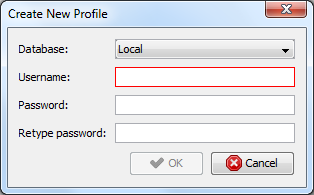
\includegraphics[scale=0.8]{images/sh_user_dialog.png}
   \caption{User Creation Dialog}
   \label{fig:user_dialog}
\end{figure}

\sh includes its own user management.
A profile is used to save personal settings and open sessions (see \subsubsecref{sec:scaffoldhunter:SessionManagement}).
To create a new user, click on the button \gui{Create User}.
Thereby the \guidialog{User Creation Dialog} shown in \figref{fig:user_dialog} is opened, where you can choose the database on which to create the user, as well as a username and password.
After clicking \gui{Ok} the program will connect to the selected database and
create a new user with the specified username. If the specified username already
exists in the database user creation will fail and an error message will be
displayed.
